% BORRADOR DE TRABAJO. Compilación: ver README.md.
\documentclass[conference,a4paper]{IEEEtran}
\usepackage[T1]{fontenc}
\usepackage[utf8]{inputenc}
\usepackage[spanish,es-nolayout,es-tabla]{babel}
\usepackage{mathptmx}
\usepackage{booktabs,array}
\usepackage{graphicx}
\usepackage{tikz}
\usetikzlibrary{arrows.meta,positioning,fit}
\usepackage[hidelinks]{hyperref}
\AddToHook{shipout/foreground}{\put(297.6,-26){\makebox(0,0)[c]{\footnotesize\sffamily BORRADOR DE TRABAJO · 5 de noviembre de 2026 · sin métricas de visión · pág.~\thepage}}}

\begin{document}
\renewcommand{\IEEEkeywordsname}{Palabras clave}
\title{Estimación de ocupación en buses a partir de eventos de conteo: arquitectura y verificación del software}
\author{\IEEEauthorblockN{Álvaro [apellido pendiente] y [compañero, nombre pendiente]}
\IEEEauthorblockA{Inteligencia Aplicada, 4.º año de Ingeniería Informática\\
{[}universidad pendiente{]}, Paraguay}}
\maketitle

\begin{abstract}
La auditoría del nivel de ocupación del transporte público del Gran Asunción requiere datos de carga por parada. Este trabajo propone un sistema que cuenta subidas y bajadas en la puerta de un bus y calcula la ocupación a lo largo de un recorrido simulado. La ruta de software ya implementada recibe eventos JSON, los asigna a paradas mediante una API REST y los muestra en un panel web, con arranque reproducible en Docker. Siete pruebas de la API y recorridos reales del navegador verificaron el cálculo, la validación y la visualización en Linux y Windows con eventos sintéticos y manuales. Estos resultados verifican el software de ocupación y no miden visión por computadora. La detección, el seguimiento y el cruce de una línea virtual siguen en desarrollo, por lo que sus métricas se incorporarán en la versión final.
\end{abstract}

\begin{IEEEkeywords}
conteo de pasajeros, ocupación, seguimiento de objetos, API REST, transporte público
\end{IEEEkeywords}

\section{Introducción y contexto}
La calidad del servicio de buses en el Gran Asunción requiere auditar las frecuencias y el nivel de hacinamiento de las unidades. Para ello no alcanza con saber cuántas personas subieron en total: una empresa o un ente de control necesita conocer la carga por parada y el porcentaje de ocupación respecto de la capacidad de la unidad. Este proyecto aborda ese problema con un módulo de visualización simulado, según la consigna de la cátedra. Este borrador no incluye cifras locales de demanda o de hacinamiento porque todavía no se contrastaron con una fuente primaria.

El conteo automático de pasajeros se investiga con distintos sensores. Hsu \emph{et al.}~\cite{hsu2020} detectan pasajeros en video de vigilancia de buses con un detector SSD y los siguen con un filtro de partículas. Seidel \emph{et al.}~\cite{seidel2022} usan en cambio datos de profundidad de LiDAR 3D, sin imágenes de personas, como alternativa respetuosa de la privacidad.

Una dificultad central del conteo por video son las oclusiones cuando varias personas cruzan a la vez, porque una identidad perdida puede duplicar u omitir un cruce. ByteTrack~\cite{zhang2022} asocia también las detecciones de baja confianza con las trayectorias existentes para recuperar objetos parcialmente ocultos. DeepSORT~\cite{wojke2017} agrega un descriptor de apariencia entrenado para reidentificación de personas, con el fin de sostener la identidad durante oclusiones largas.

La contribución actual es una ruta de software verificada desde los eventos hasta el panel, con un contrato explícito que permite integrar el módulo de visión sin modificar el cálculo de ocupación.

\section{Metodología y arquitectura del sistema}
\subsection{Arquitectura}
La Fig.~\ref{fig:arq} separa la ruta implementada del módulo de visión pendiente. Mientras ese módulo se completa, la entrada de la ruta son archivos JSON sintéticos o manuales. Las predicciones de visión deberán usar el mismo formato.

\begin{figure}[!t]
\centering
\begin{tikzpicture}[font=\scriptsize,node distance=3.5mm and 3.5mm,
  ok/.style={draw,thick,rounded corners=1pt,align=center,minimum height=6.5mm,minimum width=13mm},
  pen/.style={ok,dashed,fill=black!6},
  fl/.style={-{Latex[length=1.6mm]},thick},
  fd/.style={fl,dashed}]
\node[pen] (vid) {Clip\\de video};
\node[pen,right=of vid] (det) {Detector y\\seguimiento};
\node[pen,right=of det] (lin) {Línea\\virtual};
\node[ok,below=6mm of vid] (json) {JSON de\\eventos};
\node[ok,right=of json] (api) {API\\FastAPI};
\node[ok,right=of api] (ocu) {Ocupación\\por parada};
\node[ok,right=of ocu] (pan) {Panel\\Streamlit};
\draw[fd] (vid)--(det); \draw[fd] (det)--(lin);
\draw[fd] (lin.south) |- ++(0,-1.9mm) -| (json.north);
\draw[fl] (json)--(api); \draw[fl] (api)--(ocu); \draw[fl] (ocu)--(pan);
\node[font=\scriptsize\itshape,anchor=west] at ([xshift=2mm]lin.east) {pendiente};
\end{tikzpicture}
\caption{Ruta implementada (trazo continuo) y módulo de visión pendiente (trazo discontinuo).}
\label{fig:arq}
\end{figure}

\subsection{Contrato de eventos y datos}
Cada evento contiene \texttt{tiempo\_s}, \texttt{track\_id} y \texttt{sentido}, que vale \texttt{subida} o \texttt{bajada}. El recorrido agrega capacidad, carga inicial y paradas con su instante de inicio. Un cruce confirmado debe generar un solo evento, y un regreso en sentido contrario, uno nuevo.

Los datos disponibles son un recorrido sintético y un ensayo de oficina de 6~s tomado de un video público~\cite{video}. Ese video no muestra un bus: simula la puerta y solo sirve para ensayar la integración. Su referencia, una subida cerca de 2~s y una bajada cerca de 4~s, es un conteo manual aproximado.

\subsection{Cálculo de ocupación}
La API expone \texttt{POST /ocupacion} con FastAPI~\cite{fastapi}. Rechaza con HTTP 422 los datos inválidos, las paradas que no empiezan en 0 o no avanzan en el tiempo y los eventos desordenados. Cada parada abarca desde su inicio hasta el inicio de la siguiente. Para cada parada se calcula:
\begin{equation}
p = c_0 + s - b, \qquad o = 100\,\frac{p}{C},
\end{equation}
donde $p$ son los pasajeros acumulados, $c_0$ la carga inicial, $s$ y $b$ las subidas y bajadas acumuladas, $C$ la capacidad y $o$ la ocupación (\%). Un conteo negativo no se corrige: se conserva y genera un aviso para revisar los eventos.

\subsection{Panel y despliegue}
El panel en Streamlit~\cite{streamlit} consulta la API por HTTP. Carga recorridos JSON, permite cambiar capacidad, carga inicial e instante, y muestra indicadores, tabla y un gráfico de barras hecho con Altair~\cite{altair}. El gráfico numera las paradas, marca la última como parcial e incluye la línea del 100~\%. El cálculo y la validación permanecen en la API.

Docker Compose~\cite{compose} arranca API y panel desde una misma imagen de Python~3.12. El panel espera a que el chequeo de salud de la API sea satisfactorio.

\subsection{Integración prevista de visión}
Lo siguiente aún no está implementado en \texttt{main}. Se prevé un detector de personas preentrenado y luego ajustado con cajas anotadas, seguimiento con ByteTrack~\cite{zhang2022} y una línea virtual que emita un evento al pasar de un lado confirmado al otro. Ultralytics~\cite{ultralytics} es una opción para integrar detector y seguimiento. La elección final corresponde a la rama \texttt{vision}.

La evaluación prevista usa clips reservados y mantiene cada grabación en una sola partición. Empareja cada cruce manual con una predicción de igual sentido dentro de $\pm 1$~s y reporta F1 por sentido, error absoluto medio del conteo por clip y cuadros por segundo.

\section{Resultados y discusión}
\subsection{Verificación funcional}
La Tabla~\ref{tab:ver} resume las pruebas realizadas. Verifican el software de ocupación con eventos conocidos y no miden la capacidad de ver personas. Los 11 registros del navegador incluyen indicadores, tabla, instantes, nota parcial, presencia del gráfico, errores y avisos. Sus valores coincidieron campo por campo entre Linux y Windows.

\begin{table}[!t]
\caption{Pruebas funcionales realizadas}
\label{tab:ver}
\centering\scriptsize
\begin{tabular}{@{}>{\raggedright\arraybackslash}p{0.43\columnwidth}>{\raggedright\arraybackslash}p{0.31\columnwidth}l@{}}
\toprule
Prueba & Entorno & Resultado\\
\midrule
7 pruebas de la API (\texttt{pytest}) & Linux y Windows & 7 de 7\\
Carga de JSON en el panel, 14 registros & Linux y Windows & Coinciden\\
Gráfico y panel, 11 registros & Docker en Linux y Windows & Coinciden\\
Imagen oficial de Python 3.12 & Docker Desktop, Windows & Arranca\\
Detener y arrancar servicios & Linux y Windows & Consulta API\\
\bottomrule
\end{tabular}
\end{table}

\begin{table}[!t]
\caption{Casos de cálculo observados en el panel}
\label{tab:casos}
\centering\scriptsize
\begin{tabular}{@{}p{0.50\columnwidth}p{0.20\columnwidth}l@{}}
\toprule
Caso (capacidad, carga inicial) & Pasajeros & Ocupación\\
\midrule
Demo a 0, 5 y 10 s (20, 3) & 3, 5, 4 & 15, 25, 20~\%\\
Demo a 10 s con capacidad 40 & 4 & 10~\%\\
Segunda parada a 22 y 22,5 s (20, 3) & 5, 4 & 25, 20~\%\\
Oficina a 0, 2 y 4 s (20, 0), manual & 0, 1, 0 & 0, 5, 0~\%\\
Sobreocupación sin eventos (2, 3) & 3 & 150~\%\\
Bajada con bus vacío (20, 0) & $-1$ y aviso & $-5$~\%\\
\bottomrule
\end{tabular}
\end{table}

Los casos de la Tabla~\ref{tab:casos} muestran que la bajada ocurrida al inicio de una parada pertenece a esa parada, que el porcentaje cambia con la capacidad sin alterar el conteo y que las inconsistencias quedan visibles. Los recorridos con nombres repetidos, sin eventos y de una sola parada también dieron el resultado esperado. Las pruebas de la API no cubren el panel, y este se comprobó con recorridos automatizados del navegador. La Fig.~\ref{fig:panel} muestra el gráfico con los valores de la demo.

\begin{figure}[!t]
\centering
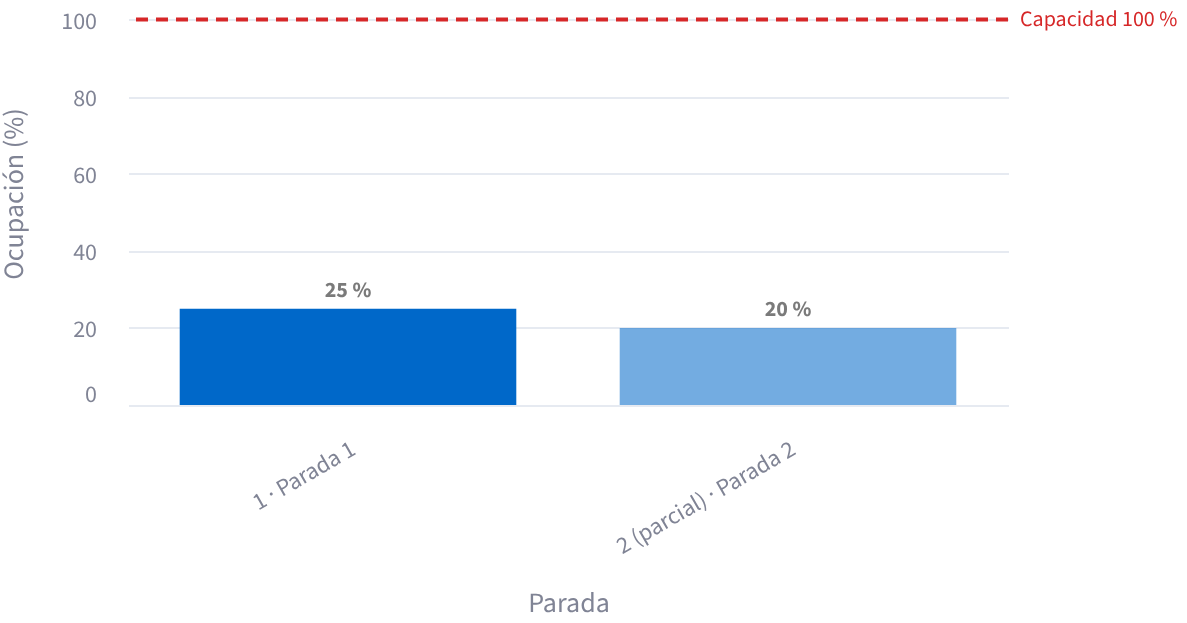
\includegraphics[width=0.92\columnwidth]{grafico-demo.png}
\caption{Gráfico del panel en la demo sintética a los 10~s. La segunda parada figura como parcial y sus valores coinciden con la tabla.}
\label{fig:panel}
\end{figure}

\subsection{Mediciones de visión}
La Tabla~\ref{tab:vis} reserva el espacio de las métricas exigidas. Sus celdas permanecerán pendientes hasta recibir la salida del evaluador de la rama \texttt{vision}. Tampoco se puede afirmar todavía funcionamiento en tiempo real: esa conclusión requiere comparar los cuadros procesados por segundo con los del video en la máquina de defensa.

\begin{table}[!t]
\caption{Métricas de visión en clips reservados (pendientes)}
\label{tab:vis}
\centering\scriptsize
\begin{tabular}{@{}lll@{}}
\toprule
Métrica & Detector base & Detector ajustado\\
\midrule
Aciertos, omisiones y falsos positivos & pendiente & pendiente\\
F1 de subidas & pendiente & pendiente\\
F1 de bajadas & pendiente & pendiente\\
Error absoluto medio por clip & pendiente & pendiente\\
Cuadros por segundo & pendiente & pendiente\\
\bottomrule
\end{tabular}
\end{table}

\begin{figure}[!t]
\centering
\fbox{\parbox[c][24mm][c]{0.9\columnwidth}{\centering\footnotesize Espacio reservado: fotograma del caso de oclusión o pérdida de identificación, con su instante y su efecto en el conteo (pendiente de visión).}}
\caption{Caso de oclusión (pendiente).}
\label{fig:oclusion}
\end{figure}

La Fig.~\ref{fig:oclusion} reserva el lugar del caso de oclusión, y este apartado deberá agregar el análisis de sus errores. Todavía no hay un caso observado.

\subsection{Discusión}
La principal decisión de diseño fue fijar el contrato antes de disponer del modelo. Eso permitió probar el cálculo con resultados conocidos y separar los errores de conteo de los errores de software. El resultado final de un clip no alcanza para validar: dos eventos omitidos pueden dar el mismo total que dos eventos correctos, por lo que la evaluación debe comparar cada cruce. Los datos actuales son sintéticos o manuales y no representan condiciones reales de un bus.

\section{Conclusiones y trabajo futuro}
La API, el contrato de eventos, el cálculo por parada, el panel, la carga de JSON y el arranque con Docker están implementados y verificados en Linux y Windows. El objetivo completo todavía no está demostrado, porque falta el conteo desde video.

Una lección del trabajo es que un contrato simple y probado permite avanzar en paralelo y mantiene visibles los errores. Las limitaciones actuales son la ausencia de eventos de visión, los datos simulados, el análisis de una sola puerta y que el recorrido se consulta por archivo y no en tiempo real.

El trabajo futuro comprende integrar el módulo de visión, evaluar el detector base y el ajustado en clips independientes, documentar un caso de oclusión y conectar el video con el contador durante la reproducción. Con clips locales se podrá estimar el desempeño en condiciones cercanas a las del Gran Asunción.

\IEEEtriggeratref{4}
\bibliographystyle{IEEEtran}
\bibliography{referencias}
\end{document}
